\documentclass{ansarticle-preprint}
%\usepackage{ucs}
\usepackage[utf8]{inputenc}
\usepackage{amsmath}
%\usepackage{cite}
\usepackage{anslistings}
\usepackage{multicol}
\usepackage{pdfsync}
\usepackage{enumitem}

\usepackage{pgfplots}
\usepackage{pgfplotstable}

\usepackage{fontenc}
\usepackage{graphicx}
\usepackage{xspace}

\usepackage{siunitx}

\usepackage{floatflt}

\usepackage{multirow}

\usepackage{booktabs}

%\renewcommand{\baselinestretch}{2.0}
%\usepackage{lineno}
%\renewcommand\linenumberfont{\normalfont\tiny}
%\linenumbers

\graphicspath{{svg/}}

\usepackage[normalem]{ulem}

\usepackage{caption}
\usepackage{subcaption}

\usepackage{todonotes}

\pgfplotsset{compat=1.9}
\definecolor{gnuplot@lightblue}{RGB}{87,181,232}
\definecolor{gnuplot@green}{RGB}{0,158,115}
\definecolor{gnuplot@purple}{RGB}{148,0,212}

\newcommand{\specialword}[1]{\texttt{#1}}
\newcommand{\dealii}{{\specialword{deal.II}}\xspace}
\newcommand{\pfrst}{{\specialword{p4est}}\xspace}
\newcommand{\trilinos}{{\specialword{Trilinos}}\xspace}
\newcommand{\aspect}{\specialword{Aspect}\xspace}
\newcommand{\petsc}{\specialword{PETSc}\xspace}
\newcommand{\snes}{{\specialword{SNES}}\xspace}
\newcommand{\ts}{{\specialword{TS}}\xspace}
\newcommand{\petscsf}{{\specialword{SF}}\xspace}
\newcommand{\cmake}{{\specialword{CMake}}\xspace}
\newcommand{\candi}{{\specialword{candi}}\xspace}
\newcommand{\MPI}{{\specialword{MPI}}\xspace}
\newcommand{\MPIx}{{\specialword{MPI+X}}\xspace}
\newcommand{\sundials}{{\specialword{SUNDIALS}}\xspace}
\newcommand{\kinsol}{{\specialword{KINSOL}}\xspace}
\newcommand{\ida}{{\specialword{IDA}}\xspace}
\newcommand{\arkode}{{\specialword{ARKODE}}\xspace}
\newcommand{\boost}{{\specialword{Boost}}\xspace}
\newcommand{\kokkos}{{\specialword{Kokkos}}\xspace}
\newcommand{\llvm}{{\specialword{LLVM}}\xspace}
\newcommand{\step}[1]{{\specialword{step-#1}}\xspace}

%Trilinos Packages
\newcommand{\epetra}{{\specialword{Epetra}}\xspace}
\newcommand{\petra}{{\specialword{Petra}}\xspace}
\newcommand{\teuchos}{{\specialword{Teuchos}}\xspace}
\newcommand{\tpetra}{{\specialword{Tpetra}}\xspace}


\usetikzlibrary{shapes.misc}
\tikzset{cross/.style={cross out, draw=black, minimum size=2*(#1-\pgflinewidth), inner sep=0pt, outer sep=0pt},
%default radius will be 1pt.
cross/.default={2pt}}

%
% Author list -- please add yourself in both places below (in
%                alphabetical order) if you think that your
%                contributions to the last release warrant this
%

\hypersetup{
  pdfauthor={
    Daniel Arndt,
    Wolfgang Bangerth,
    Maximilian Bergbauer,
    Bruno Blais,
    Marc Fehling,
    Rene Gassm\"{o}ller,
    Timo Heister,
    Luca Heltai,
    Martin Kronbichler,
    Matthias Maier,
    Peter Munch,
    Bruno Turcksin,
    David Wells,
    Michał Wichrowski,
  },
  pdftitle={The deal.II Library, Version 9.7, 2025},
}

\title{The \dealii Library, Version 9.7}

 \author[1*]{Daniel Arndt}
 \affil[1]{Computational Coupled Physics Group,
   Computational Sciences and Engineering Division,
   Oak Ridge National Laboratory, 1 Bethel Valley Rd.,
   TN 37831, USA.
   \texttt{arndtd/turcksinbr@ornl.gov}}

 \author[2,3]{Wolfgang~Bangerth}
 \affil[2]{Department of Mathematics, Colorado State University, Fort
   Collins, CO 80523, USA.
   \texttt{bangerth@colostate.edu}}
 \affil[3]{Department of Geosciences, Colorado State University, Fort
   Collins, CO 80523, USA.}

\author[4]{Maximilian~Bergbauer}
\affil[4]{Institute for Computational Mechanics, Technical University of
  Munich, Boltzmannstr. 15, 85748 Garching bei München, Germany.
  {\texttt{maximilian.bergbauer@tum.de}}}

\author[5]{Bruno Blais}
\affil[5]{Chemical Engineering High-performance Analysis, Optimization and Simulation (CHAOS) laboratory, Department of Chemical Engineering,
             Polytechnique Montréal,
             PO Box 6079, Stn Centre-Ville, Montréal, Québec, Canada, H3C 3A7.
             {\texttt{bruno.blais@polymtl.ca}}}

\author[6]{Marc~Fehling}
\affil[6]{Department of Mathematical Analysis,
    Faculty of Mathematics and Physics, Charles University,
    Sokolovsk{\'a} 49/83, 186\,75 Prague 8, Czech Republic.
    {\texttt{marc.fehling@matfyz.cuni.cz}}}


\author[7]{Rene~Gassm\"{o}ller}
\affil[7]{GEOMAR Helmholtz Centre for Ocean Research Kiel, 24148 Kiel, Germany}

\author[8]{Timo~Heister}
\affil[8]{School of Mathematical and Statistical Sciences,
   Clemson University,
   Clemson, SC, 29634, USA.
   {\texttt{heister@clemson.edu}}}

\author[9]{Luca~Heltai}
\affil[9]{Department of Mathematics, University of Pisa,
Via Buonarroti 1/c, 56127 Pisa, Italy.}

\author[10]{Martin~Kronbichler}
\affil[10]{Faculty of Mathematics, Ruhr University Bochum,
   Universit\"atsstr.~150, 44780 Bochum, Germany.
 {\texttt{martin.kronbichler@rub.de}}}

\author[11]{Matthias~Maier}
\affil[11]{Department of Mathematics,
  Texas A\&M University,
  3368 TAMU,
  College Station, TX 77845, USA.
  {\texttt{maier@math.tamu.edu}}}

\author[12]{Peter Munch}
\affil[12]{Institute of Mathematics, Technical University of Berlin, Germany.
  {\texttt{muench@math.tu-berlin.de}}}

\author[1*]{Bruno~Turcksin}

\author[13]{Siarhei Uzunbajakau}
\affil[13]{CEM Books,
  Rotterdam, The Netherlands.
  {\texttt{info@cembooks.nl}}}

\author[14]{David Wells}
\affil[14]{Department of Mathematics, University of North Carolina,
  Chapel Hill, NC 27516, USA.
  {\texttt{drwells@email.unc.edu}}}

\author[15]{Michał Wichrowski}
\affil[15]{Interdisciplinary Center for Scientific Computing, Heidelberg University, Heidelberg, Germany.
  {\texttt{mt.wichrowsk@uw.edu.pl}}}

\renewcommand{\labelitemi}{--}


\begin{document}
\maketitle

\footnotetext{%
  $^\ast$ This manuscript has been authored by UT-Battelle, LLC under Contract No.
  DE-AC05-00OR22725 with the U.S. Department of Energy.
  % We need to submit the manuscript with the text below. If the editor
  % complains we can remove it.
  The United States
  Government retains and the publisher, by accepting the article for
  publication, acknowledges that the United States Government retains a
  non-exclusive, paid-up, irrevocable, worldwide license to publish or reproduce
  the published form of this manuscript, or allow others to do so, for United
  States Government purposes. The Department of Energy will provide public
  access to these results of federally sponsored research in accordance with the
  DOE Public Access Plan (http://energy.gov/downloads/doe-public-access-plan).
}


\begin{abstract}
  This paper provides an overview of the new features of the finite element
  library \dealii, version 9.7.
\end{abstract}



%%%%%%%%%%%%%%%%%%%%%%%%%%%%%%%%%%%%%%%%%%%%%%%%%%%%%%%%%%%%%%%%%%%%%%%%%%%%%%%%
%%%%%%%%%%%%%%%%%%%%%%%%%%%%%%%%%%%%%%%%%%%%%%%%%%%%%%%%%%%%%%%%%%%%%%%%%%%%%%%%
%%%%%%%%%%%%%%%%%%%%%%%%%%%%%%%%%%%%%%%%%%%%%%%%%%%%%%%%%%%%%%%%%%%%%%%%%%%%%%%%
\section{Overview}

\dealii version 9.7.0 was released July 22, 2025.
This paper provides an
overview of the new features of this release and serves as a citable
reference for the \dealii software library version 9.7. \dealii is an
object-oriented finite element library used around the world in the
development of finite element solvers. It is available for free under the
terms of the \emph{GNU Lesser General Public License} (LGPL). The \dealii
project is in the process of relicensing the library under the terms of
the \emph{Apache License 2.0 with LLVM Exception}. Downloads are
available at \url{https://www.dealii.org/} and
\url{https://github.com/dealii/dealii}.

The major changes of this release are:
%
\begin{itemize}
\item \texttt{MappingP1}, a more efficient mapping for simplex elements
  (Section~\ref{subsec:mappingp1});

\item Updated support for transferring solution vectors during mesh refinement
  (Section~\ref{subsec:solutiontransfer});

\item Improved matrix-free support for multi-component systems as well as
  improved portability between GPUs via \texttt{Portable::MatrixFree}
  (Section~\ref{subsec:matrixfree});

\item Support for threading via TaskFlow, as well as support for
  several new external libraries and improved support for Kokkos and ArborX
  (Section~\ref{subsec:external});

\item \dealii{} can now build C++20 modules (Section~\ref{subsec:modules});

\item Three new tutorial programs and a new code gallery program
  (Section~\ref{subsec:steps}).
\end{itemize}
%
\todo[inline]{Update the list above if we add subsections to section 2.}



While all of these major changes are discussed in detail in
Section~\ref{sec:major}, there
are a number of other noteworthy changes in the current \dealii release,
which we briefly outline in the remainder of this section:
%
\begin{itemize}
\item MPGMRES is a variant of the
  widely used generalized minimal residual method (GMRES)
  \cite{Saad1986gmres}, distinguished by the support for multiple
  preconditioners (thus, \textit{MP}GMRES)  during the course of the solution process
  \cite{Greif2016gmres}. In our implementation in the
  \texttt{SolverMPGMRES} class, the use of $N$ preconditioners leads
  to the construction of multiple Krylov spaces via
  $N$-variate, non-commuting polynomials of the preconditioners and the system
  matrix applied to a residual vector. \texttt{SolverMPGMRES}
  supports two strategies: (i) a full variant that constructs all possible
  combinations of preconditioner application to the initial residual $r$,
  which for two preconditioners $P_1, P_2$ looks as
  \[
    r, P_1r, P_2r, P_1AP_1r, P_2AP_1r, P_1AP_2r, P_2AP_2r, P_1AP_1AP_1r,
   P_2AP_1AP_1r, \ldots, P_2AP_2AP_2r, \ldots;
 \]
 and (ii) a truncated version where no combinations of preconditioners are considered, i.e.
 \[
    r, P_1r, P_2r, P_1AP_1r, P_2AP_2r, P_1AP_1AP_1r,
   P_2AP_2AP_2r, \ldots.
 \]
 The new solver is beneficial when two different preconditioners can help to
 more quickly span the space in which the solution is expected.
\item A common operation in finite element codes is to ask whether
  a specific shape function belongs to a particular solution
  variable. In the past, this was implemented by using the
  \texttt{FiniteElement::system\_to\_component\_index()} function that
  returns, among other information, which vector component a shape
  function belongs to. One then had to test whether this is the vector
  component (or one of the vector components) that corresponds to a
  specific variable. The new
  \texttt{FiniteElement::shape\_function\_belongs\_to()} makes this
  easier: It takes as argument a \texttt{FiniteElementExtractor} that
  corresponds to a scalar, vector-valued, or tensor-valued set of
  solution variables, and directly returns \texttt{true} or
  \texttt{false}.
\item Most of the functions in the \texttt{GridGenerator} namespace correspond
  to simple geometries (such as cubes, spheres, and other shapes with analytical
  formulas) discretized with hypercubes. The function
  \texttt{GridGenerator::convert\_hypercube\_to\_simplex\_mesh()} converts such
  discretizations to instead use simplices. That function now supports
  anisotropic splits, including splitting quadrilaterals into two triangles and
  hexahedra into six tetrahedra, in addition to the standard isotropic splits.
  These anisotropic splits significantly reduce the total number of cells and
  are useful in contexts where one would like to use as few cells as
  possible.
\item The build system now supports interprocedural and link-time optimization
  (LTO). This can be enabled with the CMake configuration option
  \texttt{-DDEAL\_II\_WITH\_LTO=ON}. This option enables whole-program
  optimization at link-time and can make executables significantly faster.
\item \texttt{GridIn::read\_vtk()} now loads cell-centered data vectors stored
  in the input file and makes them available via
  \texttt{GridIn::get\_cell\_data()}.
\item Sparsity patterns for matrices built with \texttt{FE\_Q\_iso\_Q1} elements
  now correctly reflect the inherited sparsity on each cell, making the usage of
  this element usable as a preconditioner for a higher order problems (this is known
  as low order rediscretization, see also \cite{pazner2023low}).
  \item The assembly of ghost penalty stabilization matrices, which appear in CutFEM, can now be done 
    via \texttt{TensorProductMatrixCreator::create\_1d\_ghost\_penalty\_matrix()}. For Cartesian cells, the local penalty matrix can be constructed by exploiting the tensor-product structure   
    of the basis functions. The ghost penalty operator is expressed as 
    a Kronecker product of precomputed one-dimensional mass and penalty matrices,
    which avoids the evaluation of high-order derivatives~\cite{wichrowski2025matrix}.
    The new functionality also handles the necessary lexicographical renumbering 
    of degrees of freedom across adjacent cells via the
    \texttt{FETools::cell\_to\_face\_patch()} function.
\end{itemize}
%
The
\href{https://dealii.org/current/doxygen/deal.II/changes_between_9_6_0_and_9_7_0.html}{changelog}
-- listing more than 120
new features and bugfixes --
contains a complete record of all changes; see \cite{changes97}.



%%%%%%%%%%%%%%%%%%%%%%%%%%%%%%%%%%%%%%%%%%%%%%%%%%%%%%%%%%%%%%%%%%%%%%%%%%%%%%%%
%%%%%%%%%%%%%%%%%%%%%%%%%%%%%%%%%%%%%%%%%%%%%%%%%%%%%%%%%%%%%%%%%%%%%%%%%%%%%%%%
%%%%%%%%%%%%%%%%%%%%%%%%%%%%%%%%%%%%%%%%%%%%%%%%%%%%%%%%%%%%%%%%%%%%%%%%%%%%%%%%
\section{Major changes to the library}
\label{sec:major}

This release of \dealii contains a number of large and significant changes,
which we will discuss in this section.


%%%%%%%%%%%%%%%%%%%%%%%%%%%%%%%%%%%%%%%%%%%%%%%%%%%%%%%%%%%%%%%%%%%%%%%%%%%%%%%%
\subsection{The \texttt{MappingP1} class}
\label{subsec:mappingp1}

Classes derived from the \texttt{Mapping} base class implement
the transformation from a reference cell (such as the unit
square or reference triangle) to a concrete cell that is part of a mesh.
\dealii has supported simplex and mixed meshes since the 9.3
release~\cite{dealii93}. That release included \texttt{MappingFE}, a
\texttt{Mapping} class that uses the shape functions of a finite
element to implement this transformation; many common mappings can be
written in this way, and the class works with a variety of different elements by
delegating most computations to a \texttt{FiniteElement}
object. For example, the common bi-/trilinear mappings for quadrilaterals and
hexahedra, as well as the linear mappings on triangles and simplices,
can be implemented using \texttt{MappingFE} along with the
\texttt{FE\_Q} or \texttt{FE\_SimplexP} classes.

The current
release includes a new \texttt{MappingP1} class, which contains an optimized
implementation of the standard affine simplex mapping (i.e., the mapping from
the unit/reference cell to the real cell with a constant Jacobian on each cell). This
implementation is about six times faster than the generic one implemented in
\texttt{MappingFE}. In addition, this \texttt{Mapping} is now the default linear
mapping returned by \texttt{ReferenceCell::get\_default\_linear\_mapping()}, so
all applications which use that function for obtaining a
\texttt{ReferenceCell}-independent mapping will automatically use the more
performant class.

\subsection{Updates to the \texttt{SolutionTransfer} class}
\label{subsec:solutiontransfer}
This release extends the \texttt{SolutionTransfer} class to facilitate
the transfer of solution vectors from one mesh to another in an
adaptive mesh refinement loop, now to
all triangulation classes that support mesh refinement.
Consequently, it has subsumed the functionality of the existing
\texttt{parallel::distributed::SolutionTransfer} class, which is no
longer necessary and is now deprecated.

In the process of this update, we have also cleaned up these classes'
interfaces. In particular, some member functions, such as
\texttt{execute\_pure\_refinement()}, have been removed from the new
implementation because they provided functionality for only rarely
used cases, but substantially complicated the internal design of these
classes. To maintain prolonged support for these edge cases and to ensure
a smooth transition to the updated interface, the previous implementation
remains available in the deprecated \texttt{Legacy::SolutionTransfer} class,
which is planned for removal in a future release.


\subsection{Matrix-free functionality}
\label{subsec:matrixfree}

The current release includes several extensions, major bug fixes, and optimizations of the
matrix-free infrastructure and related multigrid functionality, such as
matrix-free geometric and polynomial coarsening. The most significant advances were made for the \kokkos-based
``portable'' infrastructure described below. In addition, improvements where
made to several areas:
\begin{itemize}
\item The \texttt{MatrixFreeTools::compute\_matrix()} and
  \texttt{MatrixFreeTools::compute\_diagonal()} functions to compute the
  matrix or only its diagonal from a matrix-free operator were extended
  towards multi-component systems, the DG context (and, in general, to operators
  with face integrals), and mixed elements.
\item We added support for additional ghost cells in the matrix-free setup to
  support vector access to a wider range of operations, such as MPI
  parallelization of multigrid smoothers based on vertex
  patches~\cite{Wichrowski2025smoothers}.
\item We implemented functionality for identifying degrees of freedom in lexicographic
  ordering on patches of cells.
\item Support for additional matrices in the
  \texttt{TensorProductMatrixCreator} class, supporting fast
  diagonalization-based inverses, was added.
\end{itemize}

In a broader context, the
\texttt{Portable::MatrixFree} class utilizes \kokkos to provide support for GPUs from
Nvidia, AMD, and Intel. In this release, we have added support for finite
elements with multiple components, i.e., ``vector-valued'' finite elements. We have
also added support for finite elements where the number
of quadrature points per direction is different from the size of the
one-dimensional basis (e.g., polynomial degree plus one), thus supporting more
cases of evaluation. In addition to the extended functionality, several
performance optimizations to the evaluation routines have been made, which are
particularly visible on recent Nvidia GPUs.

To ensure more uniform handling of data structures necessary for
storing temporary results in matrix-free evaluations, such as
sum-factorization algorithms, we have introduced two new classes:
\texttt{Portable::DeviceVector} and
\texttt{Portable::DeviceBlockVector}. The first of these is an
alias for \texttt{Kokkos::View} that replaces the raw pointer previously used
to access data on the GPU. The class \texttt{Portable::DeviceBlockVector} extends
\texttt{Portable::DeviceVector} in a manner similar to the way
\texttt{BlockVector} extends \texttt{Vector} on the CPU.

Finally, we have streamlined the interface of the functor invoked by the GPU
kernel. In the past, this interface included a cell index,
\texttt{Portable::MatrixFree::Data} (which includes precomputed data such as
quadrature points, shape functions, and other information that needs to be
transferred to the GPU), and \texttt{Portable::MatrixFree::SharedData} (which
contained scratch memory used for computation). Now, all this information has
been consolidated into a single new class
\texttt{Portable::MatrixFree::Data}, greatly simplifying the interface.

%% The major simplex additions are the changes to
%% convert_hypercube_to_simplex_mesh() and MappingP1: those are discussed
%% elsewhere so we don't need a dedicated section for the general topic

\subsection{Updates of \dealii{}'s interfaces to external libraries}
\label{subsec:external}

\dealii{} relies on external software packages for many operations
that are not within the core functionality of a finite element package
-- see Section~\ref{sec:cite} for a complete list. As in every
release, we have continued to expand and revise these interfaces. The
following sub-sections outline these updates.

\subsubsection{Interfaces to the Threading Building Blocks and to
  Taskflow}

A large number of operations within \dealii{} are parallelized,
including through mechanisms like WorkStream \cite{TKB16} that are
also available to and useful in application codes. For more than
15 years, since the 6.3 release, \dealii{} has used the Intel Threading
Building Blocks (TBB) \cite{reinders2007tbb} as the underlying library to
provide task- and pipeline-based parallelism. However, the TBB has
downsides that primarily follow from its use of assembler mnemonics
and the resulting difficulties with supporting all platforms and
compilers. As a consequence, starting with the current release,
\dealii{} builds on the Taskflow library \cite{huang2021taskflow} that
is entirely implemented in C++, is header-only, and provides an
interface that matches well with current C++ language standards. \dealii{}
bundles the Taskflow 3.10 release, and now no longer bundles the TBB,
though the TBB interfaces are still available if a TBB installation
is found on a system.

In Figure~\ref{fig:tbb-vs-taskflow} we compare the time for assembling
the temperature matrix and temperature right-hand side in the step-32
tutorial program, like it was done in \cite{TKB16}. The test was performed
on a 3d mesh with 393,216 cells and 3,195,010 temperature degrees of freedom
using a $Q_2$ element. The tests are run
on AMD EPYC 9654P with 96 cores (and 192 threads). One can clearly see that
running all copy operations sequentially limits parallel scalability (to less than 10
threads on the left, where the copy operation is more expensive than
the right), regardless of whether one uses the TBB or Taskflow. On the
other hand, first ``coloring'' all cells to avoid conflicts in
the copy operation (labeled as ``colored'' in the figure) eliminates this bottleneck.
It is clearly visible that the Taskflow implementation is better or the same
in all situations.

\begin{figure}[tb]
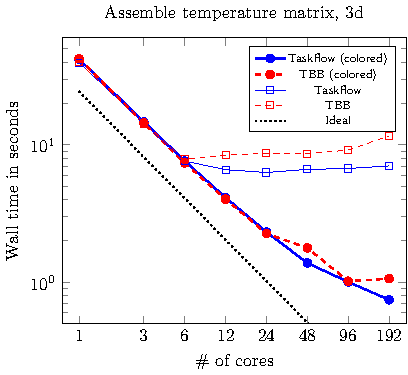
\includegraphics{taskflow-vs-tbb/plots-figure1.pdf}\hfill
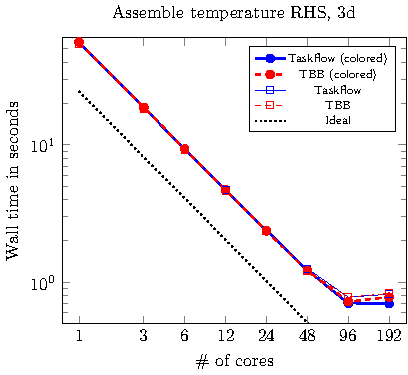
\includegraphics{taskflow-vs-tbb/plots-figure2.pdf}
\caption{Assembly times in a modified step-32 (left: temperature
  matrix assembly, right: temperature right-hand side assembly)
  comparing TBB and Taskflow with and without coloring. These figures
  correspond to the middle row of \cite[Fig. 4]{TKB16}. Lines with
  squares match ``Implementation 2'' in \cite{TKB16}; the lines with
  circles labeled ``colored'' match ``Implementation 3'' therein.}
\label{fig:tbb-vs-taskflow}
\end{figure}


\subsubsection{\kokkos, a performance portability library}
\label{subsec:external-kokkos}

\kokkos~\cite{trott2022} is a C++ library that makes it easy to write codes that can
portably run on CPUs and GPUs of different vendors, using their
respective underlying programming models.
The \dealii{} 9.5 release~\cite{dealII95} made \kokkos a required
dependency. The current release removes the deprecated \texttt{CUDAWrappers} namespace as well
as all \texttt{CUDA}-related macros in favor of \kokkos
equivalents. The 9.7 release now bundles \kokkos 4.5.1 but the minimum version required is still 3.4.

\subsubsection{MUMPS, a multifrontal parallel direct solver}

MUMPS (MUltifrontal Massively Parallel sparse direct Solver) is a
widely-used software library designed for efficiently solving large sparse linear systems on parallel architectures~\cite{amestoy2001mumps}.

In the 9.7 release, we have significantly enhanced integration with MUMPS,
without requiring it to be installed through PETSc or Trilinos. Improvements
include a simplified user interface for direct solvers, mimicking the existing
interface we provide for UMFPACK, and enhanced performance optimizations that
leverage recent MUMPS capabilities. Specifically, the deal.II wrappers now
transparently support parallel matrix factorization, out-of-core computations,
block low-rank approximations, and GPU support.

\subsubsection{PSBLAS, a parallel sparse linear algebra library}

PSBLAS is a parallel sparse linear algebra library that provides basic operations for sparse matrices and vectors~\cite{Filippone2000psblas}.

The library is specifically designed to leverage modern
parallel computing architectures, including both CPU and GPU systems, making it well-suited for exascale
computing environments. Release 9.7 includes preliminary support for configuring with PSBLAS, allowing users to take advantage of its capabilities for specific linear algebra tasks. This support is still in its early stages, and the library is not yet fully integrated into the \dealii{} ecosystem.

\subsubsection{Magic Enum, a static reflection library for enums}

Magic Enum (alternatively known via its in-code spelling \texttt{magic\_enum}) is a modern, header-only C++17 library designed to provide static reflection capabilities for enums without the need for macros or additional boilerplate code. It greatly simplifies working with enum types by enabling conversions between enum values and strings, integer values, and various other operations. Version 9.7 uses \texttt{magic\_enum} to provide type safe and efficient conversions between enum values and their string representations in the \texttt{ParameterHandler} class. An example usage of this class would be:

\begin{c++}
  #include <deal.II/base/parameter_handler.prm>

  enum class SolverType {
    DirectUMFPACK,
    DirectMUMPS,
    Iterative
  };

  SolverType solver_type = SolverType::DirectUMFPACK;
  ParameterHandler prm;
  prm.add_parameter("solver_type", solver_type);
  prm.parse_input("input.prm");
\end{c++}

This allows the user to specify in the parameter file \verb|input.prm|, e.g., the type of solver to use:
\begin{verbatim}
  set solver_type = DirectUMFPACK
\end{verbatim}

The library also understands boolean operations between enums, allowing the user to specify, for example:
\begin{c++}
  #include <deal.II/base/patterns.h>
  #include <deal.II/fe/fe_values.h>

  // This is one of the deal.II enums used for the FEValues class
  UpdateFlags flags = update_values;

  // The following will output "update_values"
  std::cout << Patterns::Tools::to_string(flags)
            << std::endl;

  // While the following is equivalent to writing 
  // flags = update_values|update_gradients;
  flags = Patterns::Tools::to_value<UpdateFlags>(
    "update_values|update_gradients");

  // Allowing one to use
  ParameterHandler prm;
  prm.add_parameter("update_flags", flags);
  prm.parse_input("input.prm");
\end{c++}

In this case, the user can specify in the parameter file \verb|input.prm| the flags to pass to an \verb|FEValues| object: 
\begin{verbatim}
  set update_flags = update_values|update_gradients
\end{verbatim}

\subsubsection{ArborX, a performance-portable geometric search library}
ArborX~\cite{prokopenko2025} is a library for geometric search on CPUs and GPUs.
The new ArborX 2.X series is not backward compatible with the older 1.X series.
Consequently, this incompatibility required an extensive rewrite of our wrappers to
support ArborX 2.X. As part of the rewrite, the template parameters had to
be changed. When using the wrappers with ArborX 1.X, \texttt{ArborX::BVH}
and \texttt{ArborX::DistributedTree} are templated on both the dimension and
the number type. When using the wrappers with ArborX 2.X, these classes are
templated on the geometric objects used for the leaf nodes of the
\texttt{ArborX::BVH} type.


\subsection{Work towards C++20 modules}
\label{subsec:modules}

\dealii{} currently requires a compiler that understands C++17, but
some additional features are enabled if a compiler supports the C++20
standard. C++20 also introduces ``modules'', a way by which software
packages can export their public interface without relying on the
mechanism of textual inclusion of header files that C++ has inherited from C. The
end goal of C++20 modules is that one can replace the use of long
lists of statements such as\\
\hspace*{1cm}\texttt{\#include <deal.II/grid/tria.h>}\\
by a simple\\
\hspace*{1cm}\texttt{import dealii;}

A lot of effort -- perhaps 6 weeks of full-time work, and nearly 200
pull requests -- has gone into evaluating whether \dealii{} can be
built using modules (in addition to header files, which will need to
be provided for a long time to come for backward compatibility). A
detailed accounting of this effort can be found in
\cite{bangerth2025experienceconvertinglargemathematical}. The majority
of this work addressed features of the \dealii{} code base,
accumulated over its more than 25 year history, that were acceptable
in a header-based system but not in a module-based system. To name
just two of many examples: (i) there can be cycles of header files that mutually
\texttt{\#include} each other, but this is not allowed for
modules; and (ii) it is allowed to declare functions in header files
as \texttt{static} or in anonymous namespaces, but this no longer
works with modules. In both cases, while allowed, the existing code
was brittle, inefficient, or hard to understand. Most of the pull requests for this project therefore simply
cleaned up our code base, without having to introduce any
incompatibilities.

As shown in \cite{bangerth2025experienceconvertinglargemathematical},
the use of C++20 modules
reduces compile times for the library itself, though the evidence is
mixed for tutorial programs or applications that build on
\dealii{}. Given that at the moment few systems have compilers, CMake
versions, and build systems that are sufficiently new to support
module builds, it will be several years before this feature will
become widely usable. However, the infrastructure for it is now
in place, and one can build the current release into a C++20 module by
providing CMake with the flag \texttt{-DDEAL\_II\_WITH\_CXX20\_MODULE=ON}.



%%%%%%%%%%%%%%%%%%%%%%%%%%%%%%%%%%%%%%%%%%%%%%%%%%%%%%%%%%%%%%%%%%%%%%%%%%%%%%%%
\subsection{New and improved tutorials and code gallery programs}
\label{subsec:steps}

Many of the \dealii tutorial programs were revised in a variety of ways
as part of this release: Around 125 of the more than 1500 (non-merge)
commits that went into this release touched the tutorial.
% data generated using these commands:
% - tutorial: git log --since 2024/08/11 --until 2025/07/19 --no-merges examples | grep commit | wc -l
% - total:    git log --since 2024/08/11 --until 2025/07/19 --no-merges | grep commit | wc -l
In addition, there are a number of new tutorial
programs:
\begin{itemize}
  \item
    \step{93}
    demonstrates how one can implement problems in which some of the
    variables to be solved for are not degrees of freedom of a finite
    element field (i.e., they are ``non-local'' degrees of freedom, because
    they have no associated node functional that is tied to a cell or
    a patch of cells). Specifically, the program solves an
    optimization problem in which some of the variables are scalars
    that multiply certain source terms.
    \step{93} was written by Sam Scheuerman.
  \item
    \step{95} extends \step{85} and illustrates the use of matrix-free methods to solve
    problems with embedded boundaries using the CutFEM method~\cite{bergbauer2025high}. 
    It shows the interplay between the matrix-free infrastructure for standard quadrature rules 
    (\texttt{FEEvaluation} / \texttt{MatrixFree}) and the infrastructure for unstructured
     quadrature (\texttt{FEPointEvaluation} / \texttt{NonMatching::MappingInfo}) while using explicit 
     \texttt{SIMD} vectorization. The tutorial implements both continuous and discontinuous Galerkin 
     methods in 2D and 3D.
    \step{95} was written by Maximilian Bergbauer, with help by Martin Kronbichler and Peter Munch.
  \item
    \step{97}
    is a program that solves a curl-curl problem from electromagnetics
    -- more specifically, from magnetostatics. The program shows a
    formulation in which two curl-curl problems are solved
    consecutively to model the magnetic field that results from the
    current in an electrically conducting coil.
    \step{97} was written by Siarhei Uzunbajakau.
\end{itemize}

In addition, there is one new program in the code gallery (a collection of
user-contributed programs that often solve more complicated problems
than tutorial programs, and that are intended as starting points for further
research rather than as teaching tools):
\begin{itemize}
  \item \emph{``Phase field fracture model in 3D''},
    contributed by Wasim Niyaz Munshi,
    Chandrasekhar Annavarapu,
    Wolfgang Bangerth, and
    Marc Fehling. The program solves a formulation for fracture
    propagation in which one uses a separate field that tracks the
    ``damage'' to the material that has resulted from deformation,
    with the damage weakening the elastic properties of the deforming solid.
\end{itemize}


%%%%%%%%%%%%%%%%%%%%%%%%%%%%%%%%%%%%%%%%%%%%%%%%%%%%%%%%%%%%%%%%%%%%%%%%%%%%%%%%
\subsection{Incompatible changes}\label{subsec:deprecated}

The 9.7 release includes
\href{https://dealii.org/developer/doxygen/deal.II/changes_between_9_6_0_and_9_7_0.html}
     {around 25 incompatible changes};
see \cite{changes97}. Many of these
incompatibilities remove previously deprecated functions or classes,
or require now widely available but newer versions of external
dependencies than previous \dealii{} versions. Others
change internal
interfaces that are not usually used in external
applications. The following are worth mentioning since they
are more broadly visible:
\begin{itemize}
  \item The classes \texttt{Subscriptor} and \texttt{SmartPointer} have been
    renamed to \texttt{EnableObserverPointer} and \texttt{ObserverPointer}. Many
    core classes, such as \texttt{DoFHandler} and \texttt{Triangulation},
    inherit from \texttt{EnableObserverPointer} to enable other classes to store
    \texttt{ObserverPointer}s pointing to them which, if dereferenced after the
    pointed-to object goes out of scope, will signal an error that the
    pointer is now ``dangling''. This
    functionality has been in \dealii since 1998. Since the term ``smart pointers''
    nowadays typically refers to the \texttt{std::unique\_ptr} or
    \texttt{std::shared\_ptr} classes, these
    names were updated to avoid this conflict in terminology. The new names are
    based on the proposal for \texttt{std::observer\_ptr}~\cite{Brown2014} and
    \texttt{std::enable\_shared\_from\_this}.

  \item In order to support modules (see Section~\ref{subsec:modules}), a
    significant number of headers had to be split up to prevent circular
    inclusions and other minor incompatibilities. For example,
    \texttt{deal.II/grid/tria.h} no longer contains declarations of \texttt{CellData} or
    \texttt{SubCellData}. Those declarations have instead been moved to
    \texttt{deal.II/grid/cell\_data.h}. In cases where this leads to errors,
    the situation is easily (and backward compatibly) fixed by adding an explicit
    \texttt{\#include} statement to the user program for the file that is necessary to
    access declarations the compiler now no longer sees.

  \item As mentioned in
    Section~\ref{subsec:external-kokkos}, the current release
    removes the deprecated \texttt{CUDAWrappers} namespace as well
    as all \texttt{CUDA}-related macros in favor of \kokkos
    equivalents.

    % This is similar to a note in the 9.6 paper, but I (David) made more
    % orientation changes for 9.7. These were done in #17988 and #18333.
  \item We have continued unifying the various implementations of object
    orientations in the library, i.e., the description of how cells,
    faces, or edges are oriented relative to other such objects. While the three booleans `orientation', `rotation',
    and `flip' have maintained their original definitions (i.e., they have default
    values of \texttt{true}, \texttt{false}, and \texttt{false}), the default
    value of the combined orientation (available via
    \texttt{TriaAccessor::combined\_face\_orientation()} and
    \texttt{TriaAccessor::line\_orientation()}) is now $0$ rather than $1$. In
    addition, the return type of these functions is now
    \texttt{types::geometric\_orientation}, which is a \texttt{typedef} for an
    8-bit integral type.

  \item The \step{52} tutorial was removed. This program showed
    the use of time stepping functionality in \dealii{}, but
    this functionality was rudimentary compared to what packages such
    as SUNDIALS or PETSc TS offer. As a consequence, \step{52} did
    not show the advanced techniques we would like to promote (e.g.,
    time stepping error control and automatic time step size choice), and it
    is now superseded by \step{86} (which builds on PETSc TS).
  \item The \texttt{parallel::distributed::SolutionTransfer} class has been
    merged with the class \texttt{SolutionTransfer}, with the
    former now being deprecated. In the process of cleaning up the
    interface, we have also removed some rarely used member functions
    of the latter that prevented us from unifying the two classes. For more
    information see Section~\ref{subsec:solutiontransfer}.
  \item The \texttt{MatrixOut} class, which creates graphical
    representations of matrices, now defaults to creating sparse
    output, only showing nonzero entries. This vastly increases the
    size of matrices that can be visualized. Creating dense output
    remains possible through a flag in the class's
    \texttt{AdditionalData} structure.
  \item The \texttt{FiniteElement} class has a number of functions
    that allow querying properties of implementations in derived
    classes. These include asking whether a derived class is able to provide
    ``(generalized) support points'', i.e., whether the element
    defines its shape functions via nodal interpolation (or via
    quadrature-based integrals) and can return an array of these
    points. These functions returned \texttt{false} for the
    \texttt{FE\_Nothing} element -- an element that has no degrees of
    freedom and consequently no shape functions. This answer was not
    wrong, but missed the point: Codes using these functions want to
    know whether an element is able to provide arrays with these
    support points, and for \texttt{FE\_Nothing} the answer should be
    ``yes'' (i.e., \texttt{true}): The class \textit{can} provide such
    an array, it will just be empty.
\end{itemize}



%%%%%%%%%%%%%%%%%%%%%%%%%%%%%%%%%%%%%%%%%%%%%%%%%%%%%%%%%%%%%%%%%%%%%%%%%%%%%%%%
%%%%%%%%%%%%%%%%%%%%%%%%%%%%%%%%%%%%%%%%%%%%%%%%%%%%%%%%%%%%%%%%%%%%%%%%%%%%%%%%
%%%%%%%%%%%%%%%%%%%%%%%%%%%%%%%%%%%%%%%%%%%%%%%%%%%%%%%%%%%%%%%%%%%%%%%%%%%%%%%%
\section{How to cite \dealii}
\label{sec:cite}

In order to justify the work the developers of \dealii put into this
software, we ask that papers using the library reference one of the
\dealii papers. This helps us justify the effort we put into this library.

There are various ways to reference \dealii. To acknowledge the use of
the current version of the library, \textbf{please reference the present
  document}. For up-to-date information and a bibtex entry
see
\begin{center}
  \url{https://www.dealii.org/publications.html}
\end{center}

The original \dealii paper containing an overview of its
architecture is \cite{BangerthHartmannKanschat2007}, and a more recent
publication documenting \dealii's design decisions is available as \cite{dealII2020design}. If you rely on
specific features of the library, please consider citing any of the
following:
\begin{multicols}{2}
  \vspace*{-36pt}
  \begin{itemize}[leftmargin=4mm]
    \item For geometric multigrid: \cite{Kanschat2004,JanssenKanschat2011,ClevengerHeisterKanschatKronbichler2019, munch2022gc};
    \item For distributed parallel computing: \cite{BangerthBursteddeHeisterKronbichler11};
    \item For $hp$-adaptivity: \cite{BangerthKayserHerold2007,fehlingbangerth2023};
    \item For partition-of-unity (PUM) and finite element enrichment methods:
           \cite{Davydov2016};
    \item For matrix-free and fast assembly techniques:
          \cite{KronbichlerKormann2012,KronbichlerKormann2019};
    \item For computations on lower-dimensional manifolds:
          \cite{DeSimoneHeltaiManigrasso2009};
    \item For curved geometry representations and manifolds:
          \cite{HeltaiBangerthKronbichlerMola2019};
    \item For integration with CAD files and tools:
          \cite{HeltaiMola2015};
    \item For boundary element computations:
          \cite{GiulianiMolaHeltai-2018-a};
    \item For the \texttt{LinearOperator} and
      \texttt{Packaged\-Operation} facilities:
          \cite{MaierBardelloniHeltai-2016-a,MaierBardelloniHeltai-2016-b};
    \item For uses of the \texttt{WorkStream} interface:
          \cite{TKB16};
    \item For uses of the \texttt{ParameterAcceptor} concept, the
          \texttt{MeshWorker::ScratchData} base class, and the
          \texttt{ParsedConvergenceTable} class:
          \cite{SartoriGiulianiBardelloni-2018-a};
    \item For uses of the particle functionality in \dealii:
      \cite{GLHPB18}.
      \item For the design of the video lectures and how they can be
        used in teaching: \cite{Zarestky2022}.
          \vfill\null
  \end{itemize}
\end{multicols}

\dealii can interface with many other libraries:
\begin{multicols}{4}
  \begin{itemize}[leftmargin=4mm]
    \item ADOL-C \cite{griewank1996adolc}
    \item ArborX \cite{prokopenko2025}
    \item ARPACK \cite{lehoucq1998arpack}
    \item Assimp \cite{schulze2021assimp}
    \item BLAS, LAPACK \cite{anderson1999lapack}
    \item Boost \cite{boost-web-page}
    \item CGAL \cite{cgal:eb-24b}
    \item Gmsh \cite{geuzaine2009gmsh}
    \item GSL \cite{galassi2009gsl,gsl-web-page}
    \item Ginkgo \cite{anzt2020ginkgo,anzt2022ginkgo}
    \item HDF5 \cite{hdf5-web-page}
    \item Kokkos \cite{trott2022}
    \item Magic Enum \cite{magic-enum-web-page}
    \item METIS \cite{karypis1998metis}
    \item MUMPS \cite{amestoy2001mumps,amestoy2019mumps}
    \item muparser \cite{muparser-web-page}
    \item OpenCASCADE \cite{opencascade-web-page}
    \item p4est \cite{burstedde2011p4est}
    \item PETSc \cite{petsc-user-ref,petsc-web-page}
    \item PSBLAS \cite{Filippone2000psblas}
    \item ROL \cite{ROL2022ICCOPT}
    \item ScaLAPACK \cite{blackford1997scalapack}
    \item SLEPc \cite{roman2023improvements}
    \item SUNDIALS \cite{gardner2022enabling}
    \item SymEngine \cite{symengine-web-page}
    \item Taskflow \cite{huang2021taskflow}
    \item TBB \cite{reinders2007tbb}
    \item Trilinos \cite{mayr2025trilinos,trilinos-web-page}
    \item UMFPACK \cite{davis2004umfpack}
    \item VTK \cite{vtk-web-page}
    \item zlib \cite{zlib-web-page}
  \end{itemize}
\end{multicols}
Please consider citing the appropriate references if you use
interfaces to these libraries.

The two previous releases of \dealii can be cited as
\cite{dealII95,dealII96}.


\section{Acknowledgments}

\dealii is a worldwide project with dozens of contributors around the
globe. Other than the authors of this paper, the following people
contributed code to this release:\\

\todo[inline]{Remove all who we promoted to authors of this paper from
  the following list.}

\begin{quote}
%  authors removed:
%  Daniel       Arndt,
%  Wolfgang     Bangerth,
%  Bruno        Blais,
%  Marc         Fehling,
%  Rene         Gassmoeller,
%  Timo         Heister,
%  Luca         Heltai,
%  Martin       Kronbichler,
%  Matthias     Maier,
%  Peter        Munch,
%  Jean-Paul    Pelteret,
%  Bruno        Turcksin,
%  Siarhei      Uzunbajakau,
%  David        Wells,
%  Michał       Wichrowski,
Pasquale     Africa,
Henry        Arhin,
Maximilian   Bergbauer,
Alfredo      Buttari,
Bruna        Campos,
Nicholas     Cantrell,
Xiaoming     Cao,
Chayapol     Chaoveeraprasit,
Jerett       Cherry,
Dario        Coscia,
John         Coughlin,
Nikita       Daniliuk,
Crystal      Farris,
Marco        Feder,
Emmanuel     Ferdman,
Federico     Fernandez,
Olivier      Gaboriault,
Mohamad      Ghadban,
Mahdi        Gharehbaygloo,
Robin        Görmer,
Davit        Gyulamiryan,
Lóránt       Hadnagy,
Fernando     Herrera,
Robin        Hiniborch,
Quang        Hoang,
Jordan       Hoffart,
Sascha       Hofstetter,
Yimin        Jin,
Yann         Jobic,
Sean         Johnson,
Vaishnavi    Kale,
Sebastian    Kinnewig,
Andreas      Koch,
Jason        Landini,
Zhou         Lei,
Yingli       Li,
Nils         Margenberg,
Oreste       Marquis,
Ryan         Moulday,
Nils         Much,
Tileuzhan    Mukhamet,
Wasim~Niyaz  Munshi,
Natalia      Nebulishvili,
Luz          Paz,
David        Pecoraro,
Davide       Polverino,
Sanjeeb      Poudel,
Guilhem      Poy,
Laura        Prieto~Saavedra,
Sebastian    Proell,
Andreas      Ritthaler,
Mayank       Sabharwal,
Sam          Scheuerman,
Magdalena    Schreter,
Richard      Schussnig,
Kyle         Schwiebert,
Marc         Secanell,
Qingyuan     Shi,
Wyatt        Smith,
Simon        Sticko,
Dominik      Still,
Edward       Terrell,
Jan~Philipp  Thiele,
Xiaochuan    Tian,
Mikael       Vaillant,
Vinayak      Vijay,
Stephan      Voss,
Simon        Wiesheier,
Yi-Yung      Yang,
\end{quote}
Their contributions are much appreciated -- this project lives by its
community of users and contributors!

This release contains patches written in and contributed from
Antarctica. As a consequence, \dealii{} now consists of work written
on all seven continents.

\bigskip

\dealii and its developers are financially supported through a
variety of funding sources:

\todo[inline]{Everyone please update as appropriate.}
D.~Arndt and B.~Turcksin: Research sponsored by the Laboratory Directed Research and
Development Program of Oak Ridge National Laboratory, managed by UT-Battelle,
LLC, for the U. S. Department of Energy and supported by the U.S. Department of Energy,
Office of Science, Office of Advanced Scientific Computing Research,
Next-Generation Scientific Software Technologies program, under contract
number DE-AC05-00OR22725.

W.~Bangerth was partially supported by the National Science Foundation
under awards OAC-1835673, EAR-1925595, and OAC-2410847.

W.~Bangerth, T.~Heister, and R.~Gassm\"{o}ller were partially
supported by the Computational Infrastructure for Geodynamics initiative
(CIG), through the National Science Foundation (NSF) under Award
No.~EAR-2149126 via The University of California -- Davis.

M.~Bergbauer was supported by the German Research Foundation (DFG) under the
project ``High-Performance Cut Discontinuous Galerkin Methods for Flow
Problems and Surface-Coupled Multiphysics Problems'' Grant Agreement
No.~456365667.

B.~Blais was supported by the National Science and Engineering Research Council of Canada (NSERC)  through the RGPIN-2020-04510 Discovery Grant and the MMIAOW Canada Research Level 2 in Computer-Assisted Design and Scale-up of Alternative Energy Vectors for Sustainable Chemical Processes.

M.~Fehling was partially supported by the ERC-CZ grant LL2105 CONTACT,
funded by the Czech Ministry of Education, Youth and Sports. He was also
partially supported by the Charles University Research Centre Program No.\@ UNCE/24/SCI/005.

R.~Gassm\"{o}ller was also partially supported by NSF Awards EAR-1925677
and EAR-2054605.

T.~Heister was also partially supported by NSF Awards OAC-2015848, EAR-1925575, and OAC-2410848.

L.~Heltai is a member of Gruppo Nazionale per il Calcolo Scientifico (GNCS) of
Istituto Nazionale di Alta Matematica (INdAM). LH was partially supported by
the Italian Ministry of University and Research (MUR), under the grant MUR PRIN
2022 No. 2022WKWZA8 ``Immersed methods for multiscale and multiphysics problems
(IMMEDIATE)'', and acknowledges the MIUR Excellence Department Project awarded
to the Department of Mathematics, University of Pisa, CUP I57G22000700001.

M.~Kronbichler was partially supported by the
German Federal Ministry of Research, Technology and Space, project
``PDExa: Optimized software methods for solving partial differential
equations on exascale supercomputers'', grant agreement No. 16ME0637K.

M.~Kronbichler and L.~Heltai were partially supported by the European Research
Council (ERC) under the European Union's Horizon 2020 research and innovation
programme (call HORIZON-EUROHPC-JU-2023-COE-03, grant agreement No. 101172493
``dealii-X: an Exascale Framework for Digital Twins of the Human Body'').

M.~Maier was partially supported by NSF Award DMS-2045636 and by the
Air Force Office of Scientific Research under grant/contract number
FA9550-23-1-0007.

D.~Wells was supported by NSF Award OAC-1931516.

Charles University is acknowledged for providing computing time on the Sn\v{e}hurka cluster.

This research used in part resources on the Palmetto Cluster at Clemson University under National Science Foundation awards MRI 1228312, II NEW 1405767, MRI 1725573, and MRI 2018069. The views expressed in this article do not necessarily represent the views of NSF or the United States government.

\bibliography{paper}{}
\bibliographystyle{abbrv}

\end{document}
